%!TEX program = xelatex
%!TEX options=--shell-escape
\documentclass[12pt]{article}

%
\usepackage[scheme=plain]{ctex}
%
\usepackage{fontspec}
%
\usepackage[margin = 1in]{geometry}

%
\usepackage[dvipsnames]{xcolor}
\usepackage[many]{tcolorbox}

%
\usepackage{amsmath}
\usepackage{amssymb}
\usepackage{amsthm}
%
\usepackage{tensor}
%
\usepackage{slashed}
\usepackage{physics}
\usepackage{simpler-wick}

%
\usepackage[version=4]{mhchem}

%
\usepackage{mathtools}

%
\usepackage{bm}
\newcommand{\dbar}{\dif\hspace*{-0.18em}\bar{}\hspace*{0.2em}}
\DeclareMathAlphabet\mathbfcal{OMS}{cmsy}{b}{n}
%\usepackage{bbold}
\newcommand*{\dif}{\mathop{}\!\mathrm{d}}
\newcommand*{\euler}{\mathrm{e}}
\newcommand*{\imagi}{\mathrm{i}}

\renewcommand{\vec}[1]{\boldsymbol{\mathbf{#1}}}

\usepackage{caption}
\usepackage{multirow}
\usepackage{enumitem}

%
\usepackage{mathrsfs}
\usepackage{dsfont}

%
\usepackage{hyperref}
\hypersetup{
    colorlinks=true,
    linkcolor=violet,
    filecolor=blue,
    urlcolor=blue,
    citecolor=cyan,
}

%
\usepackage{graphicx}
\usepackage{subfig}
%
\graphicspath{{figures/}{../figures/}}


%
\usepackage{indentfirst}
%
\setlength{\parindent}{2em}
\linespread{1.25}

%
% \setmainfont{Times New Roman}

\title{Note}
\author{Feng-Yang Hsieh}
\date{}

\begin{document}
\maketitle


\section{Bootstrapping}% (fold)
\label{sec:bootstrapping}
    The bootstrapping method involves an iterative process of training a classifier on mixed datasets. We start by training a classifier on the initial mixed datasets. The trained classifier is then used to reclassify the data, creating a new mixed training set. This process is repeated multiple times to increase the sample fraction differences in mixed datasets. We want to explore whether this process can improve CWoLa's performance.
    
    We consider the events sampled from the normal distribution for the testing and implement this method. We found this method is unsuccessful. The model initially achieved the best performance, then worsened at subsequent iterations.

    The reason is the reclassification step breaks the key assumption of the CWoLa approach: the signal and background events should have the same distributions in both mixed datasets. Figure~\ref{fig:bootstrapping_signal_background_distribution_origin} shows the initial signal and background distributions. Signal has the same distribution in mixed dataset $M_1$ and $M_2$, as does the background. Figure~\ref{fig:bootstrapping_signal_background_distribution_iteration_1} shows signal and background distributions after the reclassification. We could observe the signal events have different distributions in $M_1$ and $M_2$. As a result, the assumption of the CWoLa approach is violated, leading to the bootstrapping method failure.
    \begin{figure}[htpb]
        \centering
        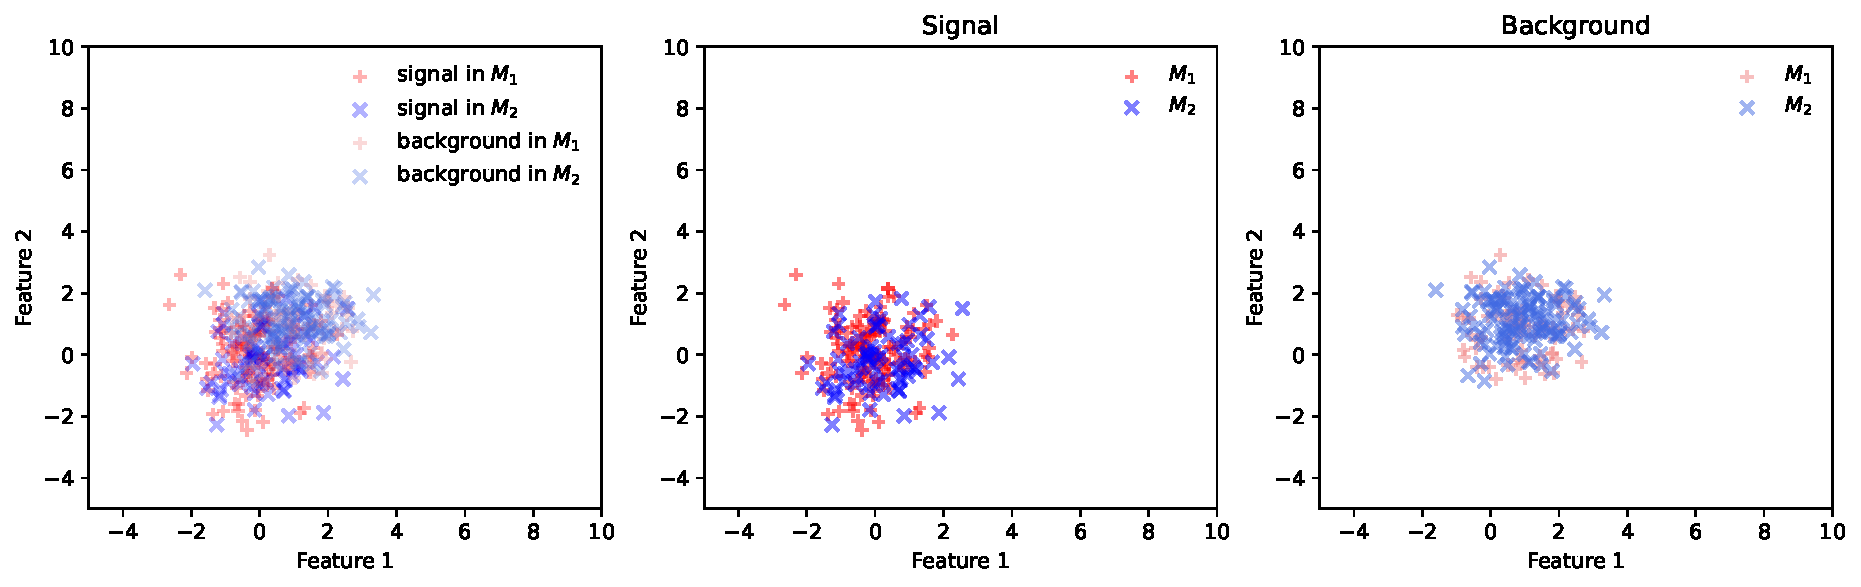
\includegraphics[width=0.97\textwidth]{bootstrapping_training_data_original.pdf}
        \caption{The signal and background samples distributions. The signal and background events are sampled from different two-dimensional normal distributions. They are randomly assigned to the mixed datasets $M_1$ or $M_2$.}
        \label{fig:bootstrapping_signal_background_distribution_origin}
    \end{figure}
    \begin{figure}[htpb]
        \centering
        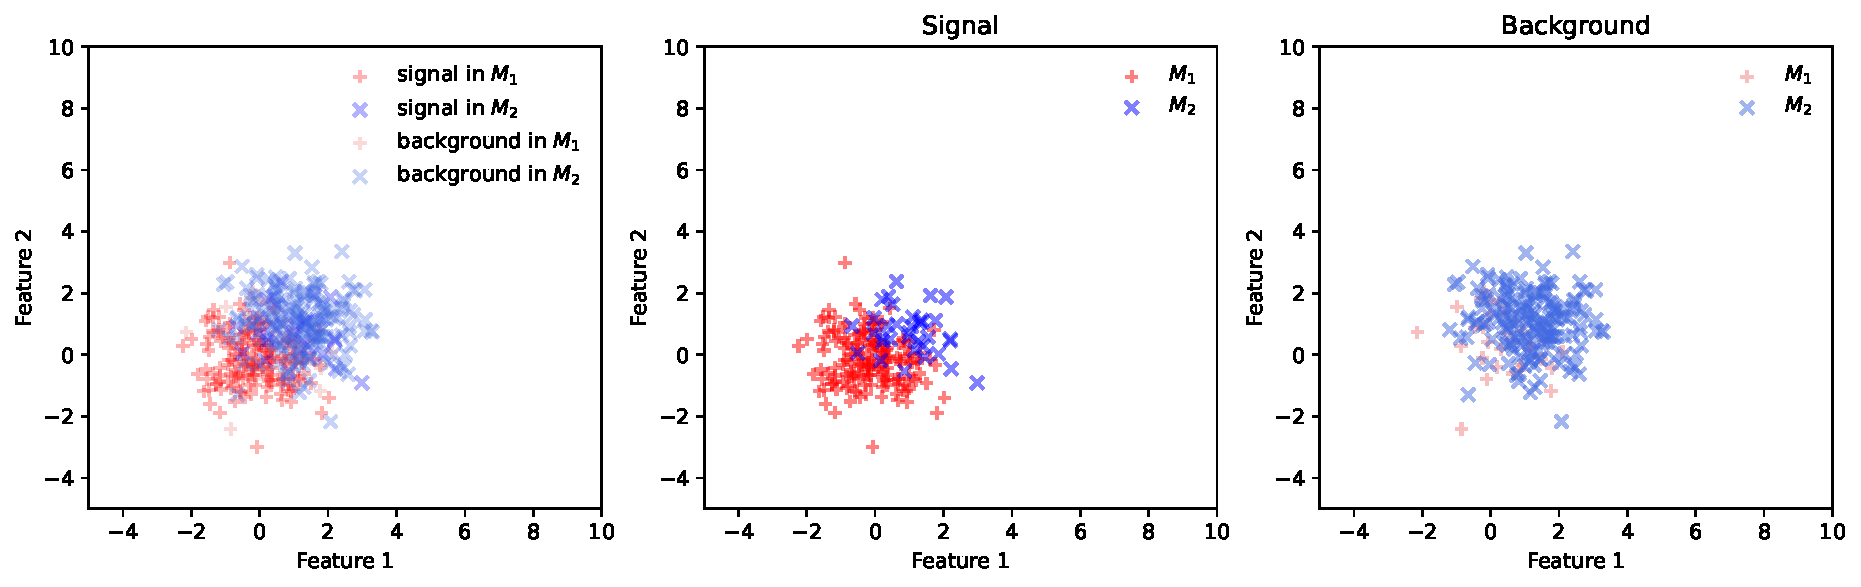
\includegraphics[width=0.97\textwidth]{bootstrapping_training_data_iteration_1.pdf}
        \caption{The signal and background samples distributions. The signal and background events are sampled from different two-dimensional normal distributions. They are assigned to the $M_1$ or $M_2$ by the trained classifier.}
        \label{fig:bootstrapping_signal_background_distribution_iteration_1}
    \end{figure}

% section bootstrapping (end)

\end{document}
